% Isto é um exemplo de Folha de aprovação, elemento obrigatório da NBR
% 14724/2011 (seção 4.2.1.3). Você pode utilizar este modelo até a aprovação
% do trabalho. Após isso, substitua todo o conteúdo deste arquivo por uma
% imagem da página assinada pela banca com o comando abaixo:
%
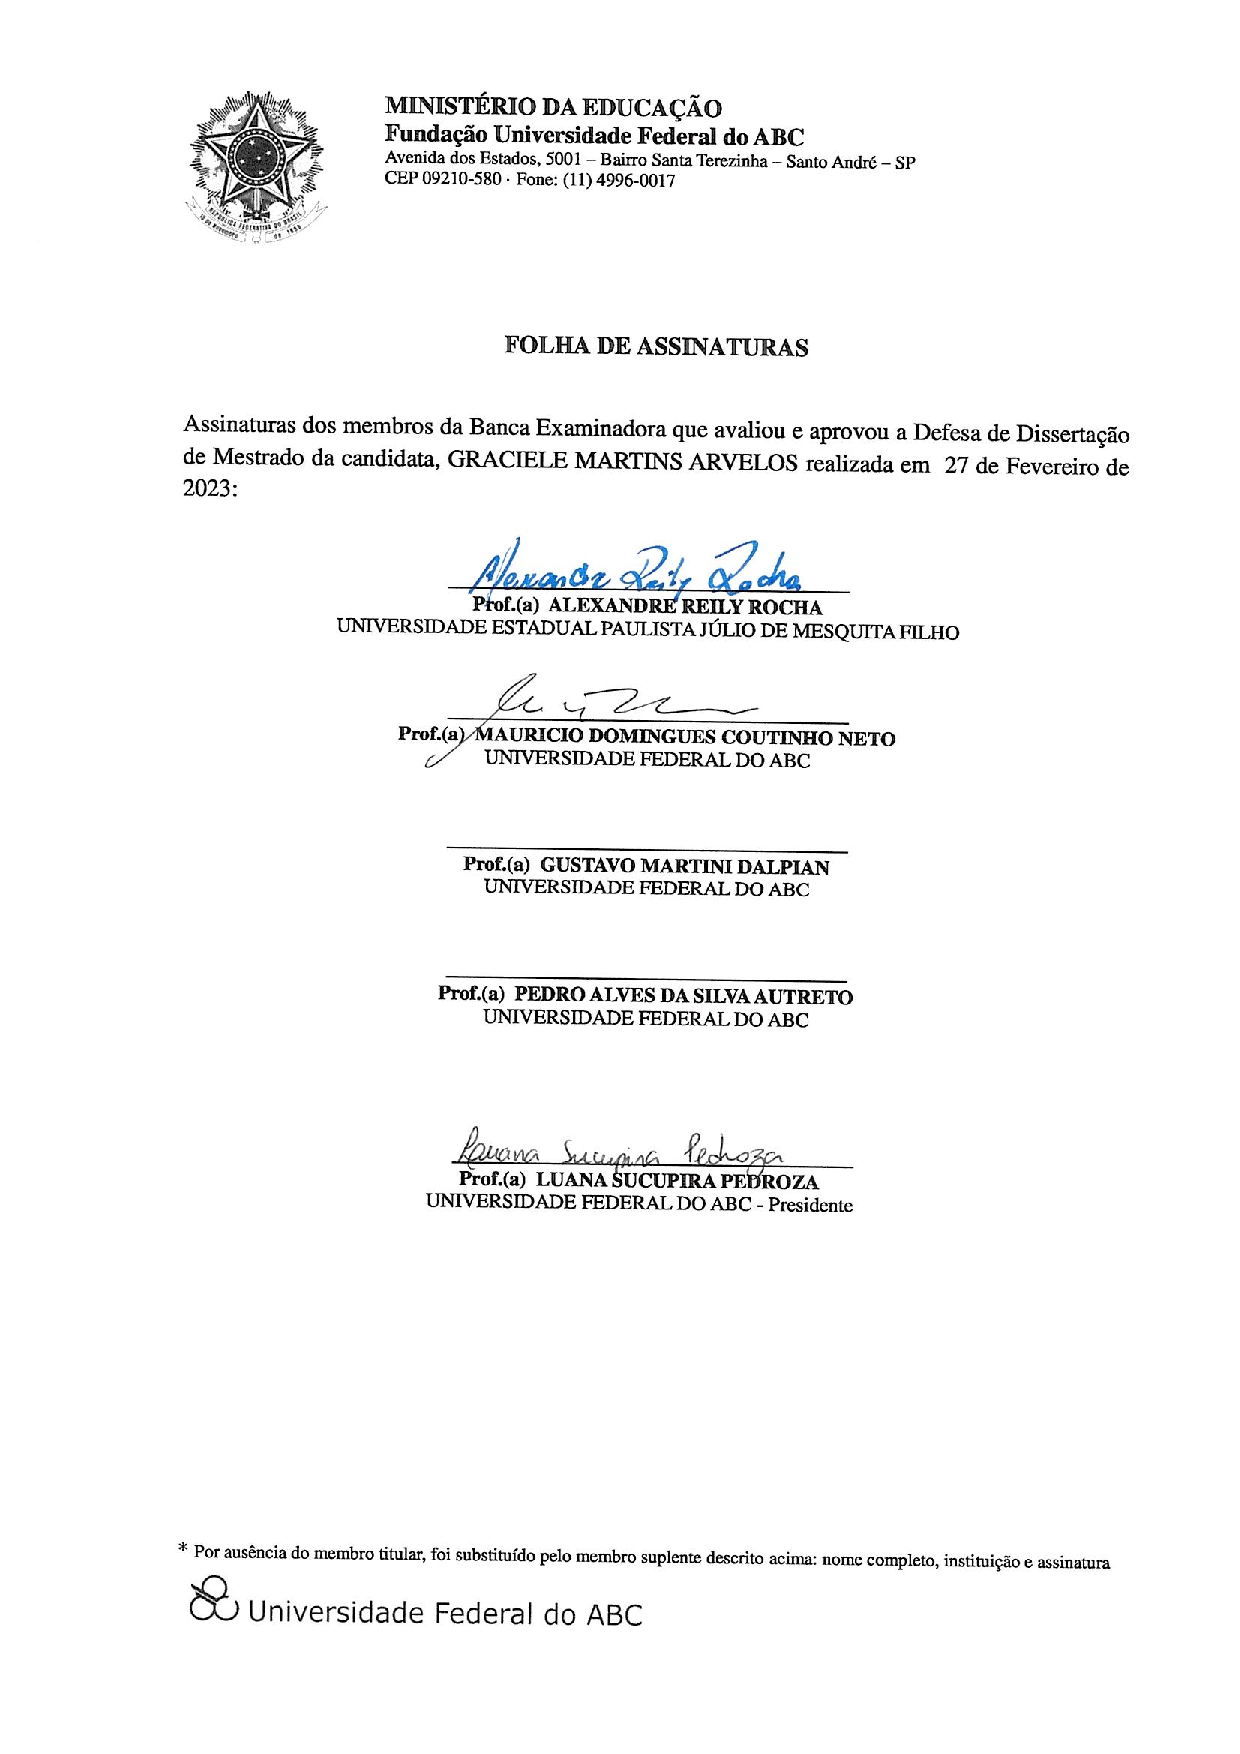
\includepdf{assinatura.pdf}
%



%\begin{folhadeaprovacao}
%
%  \begin{center}
%    {\ABNTEXchapterfont\large\imprimirautor}
%
%    \vspace*{\fill}\vspace*{\fill}
%    {\ABNTEXchapterfont\bfseries\Large\imprimirtitulo}
%    \vspace*{\fill}
%    
%    \hspace{.45\textwidth}
%    \begin{minipage}{.5\textwidth}
%        \imprimirpreambulo
%    \end{minipage}%
%    \vspace*{\fill}
%   \end{center}
%    
%   Trabalho aprovado. \imprimirlocal, \imprimirdata:
%
%   \assinatura{\textbf{\imprimirorientador} \\ Orientador} 
%   \assinatura{\textbf{Prof.$ \ulo $ Dr. Alexandre Reily Rocha}}
%   \assinatura{\textbf{Prof.$ \ulo $ Dr. Maurício Domingues Coutinho Neto}}
%   \assinatura{\textbf{Professor} \\ Convidado 3}
%   \assinatura{\textbf{Professor} \\ Convidado 4}
%      
%   \begin{center}
%    \vspace*{0.5cm}
%    {\large\imprimirlocal}
%    \par
%    {\large\imprimirdata}
%    \vspace*{1cm}
%  \end{center}
%  
%\end{folhadeaprovacao}
% ---